\chapter{Object Design}\label{ch:object_design}
In chapter \ref{ch:analysis}, we identified the objects in our system by creating the analysis object model. In chapter \ref{ch:system_design}, we mapped our objects to components and we defined the hardware and software platforms that host those components.

During hardware/software mapping, off-the-shelf components that we used throughout our system have been identified. In this chapter, we close the gap between the application objects and the off-the-shelf components by identifying additional solution objects and refining existing objects \cite{bruegge2004object}.

Section \ref{sec:artec} presents the Artec Space Spider 3D scanner and the Artec Studio 3D scanning software. It also describes how they are used to create 3D models. Section \ref{sec:rhino} presents the 3D modeling software Rhinoceros and how it is used to create synthetic images. Section \ref{sec:pillow} describes Pillow the python imaging library, and how it is used to process real images. In section \ref{sec:keras}, we introduce Keras and Tensorflow, and we describe how they are used to create an image classifier. Section \ref{sec:vgg_algorithm} describes the VGG convolutional neural network algorithms used to implement the CNNModel. Finally, Section \ref{sec:adam_algorithm} presents the Adam optimization algorithm.


\section{Artec Space Spider and Artec Studio}\label{sec:artec}
Artec Space Spider\footnote{https://www.artec3d.com/portable-3d-scanners/artec-spider} is a high-resolution 3D scanner based on blue light technology. It is built for capturing small objects or intricate details of large industrial objects in high resolution, with steadfast accuracy and precise color.

Artec Studio\footnote{https://www.artec3d.com/3d-software/artec-studio} is a 3D scanning and data processing software. It is used hand in hand with the Artec Space Spider 3D scanner to create 3D models.

\subsection{Usage}
We use the Artec Space Spider 3D scanner to scan our small part from multiple angles. The different scans are then sent to Artec Studio for processing. Artec Studio provides a functionality that detects features in multiple scans and automatically combines the scans to form a 3D model. Moreover, Artec Studio automatically removes outlier points in the scans and. We also used Artec Studio to identify the horizontal plane where the small part was lying during the scan. The plane is then removed from the output 3D model. After the scans have been combined to construct a 3D model, Artec Studio automatically fills the holes in the object where there are missing scans.


\section{Rhinoceros}\label{sec:rhino}
Rhinoceros\footnote{https://www.rhino3d.com} (Rhino for short) is a 3D modeling software. Rhino can create, edit, analyze, document, render, animate, and translate curves, surfaces, solids, point clouds, and polygon meshes.

We choose Rhino to create our synthetic data because it has a python library called \textit{RhinoScriptSyntax}. RhinoScriptSyntax provides an API for object transformation, scene manipulation and image rendering in python. Moreover, the Rhino software hosts a python interpreter and consequently supports running python scripts directly in the software. RhinoScriptSyntax and the hosted python interpreter are used to automate repetitive tasks that can otherwise consume more time if executed manually.

\subsection{Usage}
We use Rhino to create our synthetic scene. We set the background and the lighting conditions of the environment, then we import our 3D model and place it horizontally on the background.

Furthermore, RhinoSyntaxScript over python to is used to create our synthetic images. After setting up the synthetic scene in Rhino, we write a python script that executes random transformations over our 3D model. Next, a RhinoSyntaxScript function that renders and saves a 2D image is applied to the synthetic scene. In the python script, the desired number of output images is specified. Rhino repeats the transformation and rendering process accordingly.


\section{Pillow}\label{sec:pillow}
Pillow is a python imaging library built on top of PIL (Python Imaging Library). Pillow is used for image manipulation in python. The \textit{Image} module provided by Pillow has a function to open an existing image, resize it and save the new resized image. We use the Image module to implement our RealImageProcessor.


\section{Keras and Tensorflow}\label{sec:keras}
Keras is a high-level neural networks API, written in Python and capable of running on top different backends such as Tensorflow, CNTK or Theano \cite{chollet2015keras}. Keras focuses on being a user friendly API. It minimizes the number of actions required to develop common neural networks. Furthermore, Keras is designed modularly. Neural layers, optimizers, cost functions and regularization schemes are shipped as standalone components that can be easily used to create new models.

Our system runs Keras over Tensorflow. Tensorflow is an open source software library for high performance numerical computation and a machine learning framework \cite{tensorflow2015-whitepaper}. Tensorflow is a flexible library that can be used to express neural network algorithms in a wide variety of domains.

\subsection{Usage}
Keras provides an out-of-the-box implementation of different CNN models, optimizers and cost functions. We took advantage of Keras's modular components to build and fine tune our CNN models and their respective optimizers with ease.

Furthermore, Keras provides an image loader, called \textit{ImageDataGenerator}. ImageDataGenerator feeds the training, validation and testing data to the CNN models from a folder directory. Consequently, we built our DatasetSplitter using Keras's image loader.


\section{VGG CNN Algorithm}\label{sec:vgg_algorithm}
VGG is a convolutional neural network model created in 2014 by Karen Simonyan and Andrew Zisserman of the University of Oxford \cite{simonyan2014very}. VGG was introduced in the ILSVRC 2014 competition, where the team came second on the image classification benchmark with a 7.3\% error rate.

As shown in figure \ref{fig:VGG_architectures}, the VGG CNN algorithm has different configurations. For example configuration D has 16 layers while E has 19 layers. The convolution layers used in the VGG network use a 3x3 filter with a stride and a pad of 1, while the maxpooling layers use a 2x2 filter with a stride of 2.

Figure \ref{fig:VGG_architectures} shows the different VGG architecture configurations presented by Simonyan and Zisserman \cite{simonyan2014very}. We use configurations D and E to implement our CNNModel. We refer to them as \textbf{VGG16} and \textbf{VGG19} respectively.

\begin{figure}[H]
\centering
  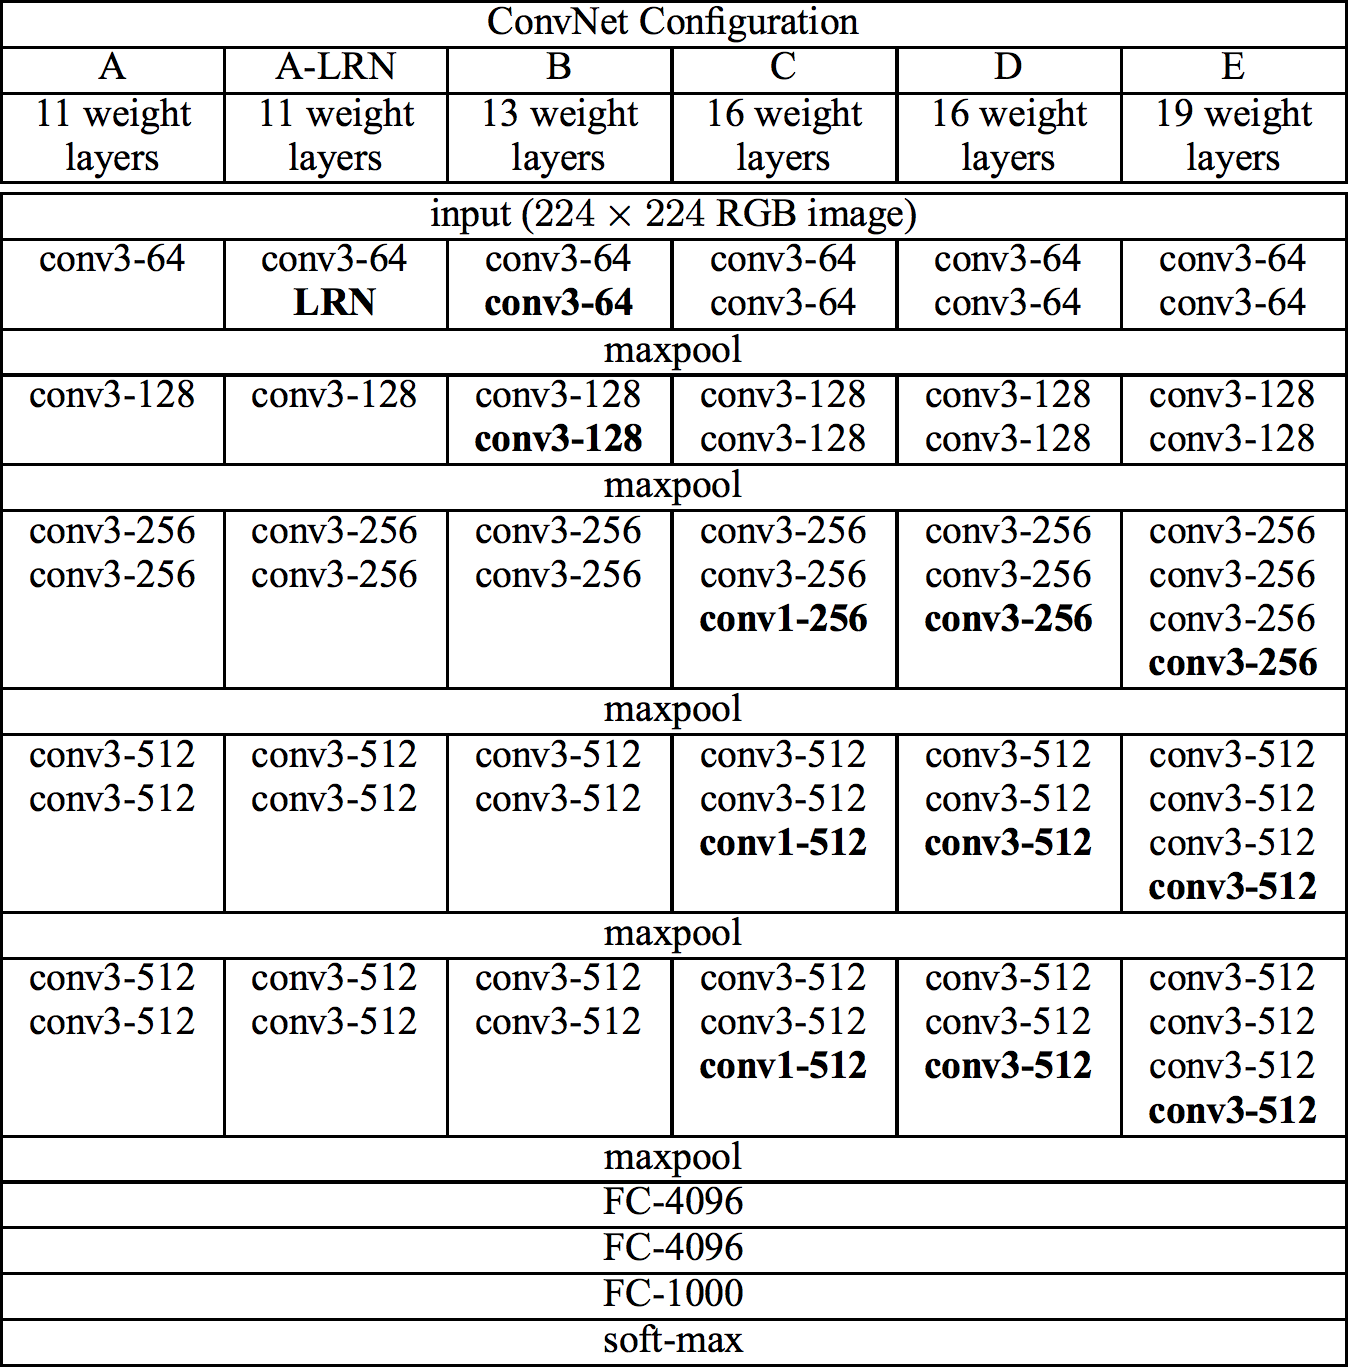
\includegraphics[width=\textwidth]{VGG_architectures}
\caption{Different VGG architectures. We use configurations D and E.}
\label{fig:VGG_architectures}
\end{figure}


\section{Adam Optimization Algorithm}\label{sec:adam_algorithm}
Adam \cite{kingma2014adam} is a gradient descent optimization algorithm. It is used during the training phase of a network to update the model weights. Adam differs than the classical stochastic gradient descent (SGD) optimizer. While SGD maintains a constant learning rate for all weight updates, Adam calculates the exponential moving average of the gradient and the squared gradient. The adam optimizer updates the weight of a network that uses the loss function $L$ as follows:
\[g_{t}=\dfrac{\partial L}{\partial w_{t-1}}\]
\[m_{t}=\beta_{1}\cdot m_{t-1}+(1-\beta_{1}\cdot g_{t})\]
\[s_{t}=\beta_{2}\cdot s_{t-1}+(1-\beta_{2}\cdot g_{t}^2)\]
\[\hat{m_{t}}=\dfrac{m_{t}}{1 - \beta_{1}^t}\]
\[\hat{s_{t}}=\dfrac{s_{t}}{1 - \beta_{2}^t}\]
\[w_{t}=w_{t-1}-\alpha\dfrac{\hat{m_{t}}}{\sqrt{\hat{s_{t}}}+\epsilon}\]

where $\alpha$ is the learning rate, $\beta_1$ and $\beta_2$ are decay rates for the moving average of the gradient and the square gradient respectively, $t$ is a timestep that starts at 0 and $\epsilon$ is a small constant (usually $10^{-8}$) used to avoid division by zero.

The Adam optimization algorithm is more sophisticated than the classical stochastic gradient descent. However, we use both algorithms to implement the Optimizer class, which is in turn used to update the weights of the CNNModel during the training phase.
